% !TEX root = ../main.tex

\section{Other Observations}

\subsection{Association Elements} \label{sec:associationelements}
	Going through the alphabet I was able to find 13 patterns that matched a letter from the alphabet. Out of the 13 letters it was 9 that had a significant number of appearances in the sample data. 

  By iterating through a list of sequences forming a patter I was able to find 385 patterns in the dataset matching one of the 13 letters in the alphabet. Compared to the total number of patterns (3393), 11.4\% of the patterns in the data set are forming a letter.

  \clearpage

    \begin{figure}[H]
      \centering
      \vspace{1.5cm}

      \subfigure[The letter C]{
        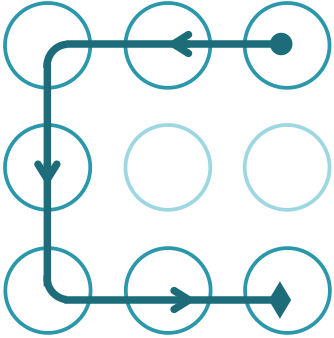
\includegraphics[width=0.27\textwidth]{pics/letters/bokstavenC.png}\hspace{0.6cm}
      }
      \subfigure[The letter L (big)]{
        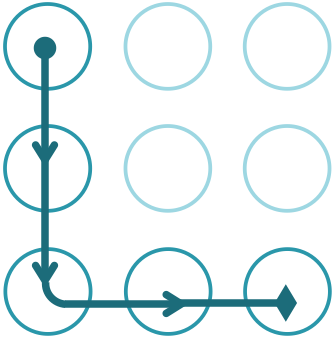
\includegraphics[width=0.27\textwidth]{pics/letters/bokstavenL.png}\hspace{0.6cm}
      }
      \subfigure[The letter L (small)]{
        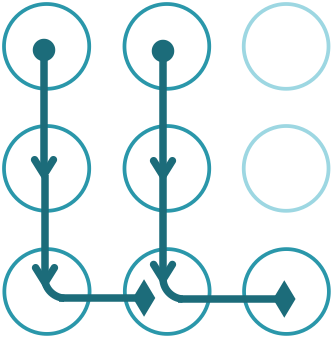
\includegraphics[width=0.27\textwidth]{pics/letters/bokstavenLitenL.png}
      }

      \vspace{0.5cm}

      \subfigure[The letter M]{
        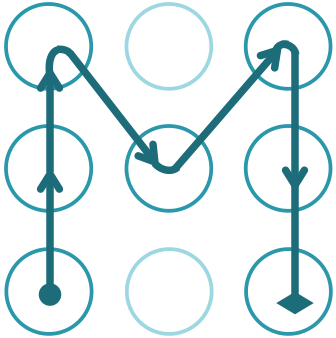
\includegraphics[width=0.27\textwidth]{pics/letters/bokstavenM.png}\hspace{0.6cm}
      }
      \subfigure[The letter N]{
        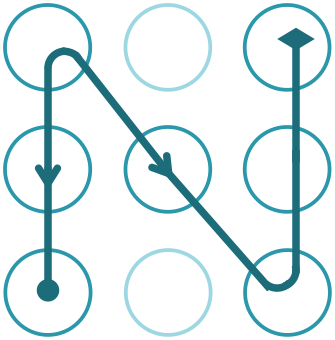
\includegraphics[width=0.27\textwidth]{pics/letters/bokstavenN.png}\hspace{0.6cm}
      }
      \subfigure[The letter O]{
        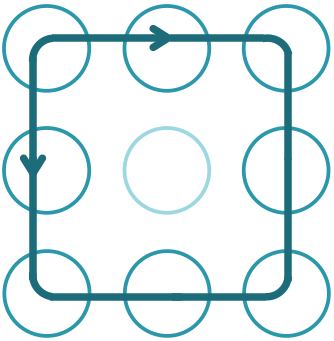
\includegraphics[width=0.27\textwidth]{pics/letters/bokstavenO.png}
      }

      \vspace{0.5cm}

      \subfigure[The letter S]{
        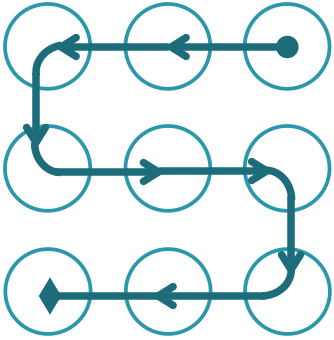
\includegraphics[width=0.27\textwidth]{pics/letters/bokstavenS.png}\hspace{0.6cm}
      }
      \subfigure[The letter U]{
        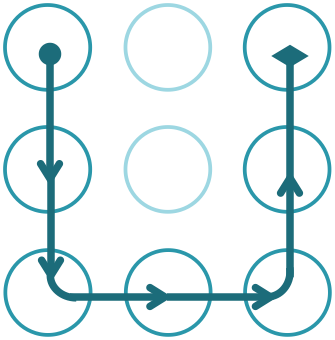
\includegraphics[width=0.27\textwidth]{pics/letters/bokstavenU.png}\hspace{0.6cm}
      }
      \subfigure[The letter Z]{
        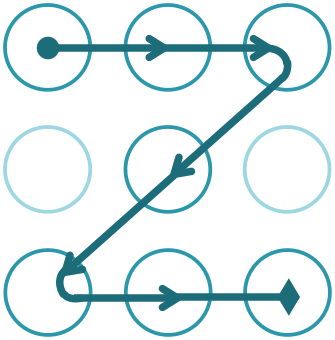
\includegraphics[width=0.27\textwidth]{pics/letters/bokstavenZ.png}
      }

      \vspace{0.5cm}
      \caption{Most frequent patterns forming letters from the alphabet}
    \end{figure}

  \clearpage

\subsection{3-gram Analysis} \label{sec:3gram}
    
  %Figure: Most common 3-gram to less common 3-gram
  \begin{figure}[H]
    \subfigure{
      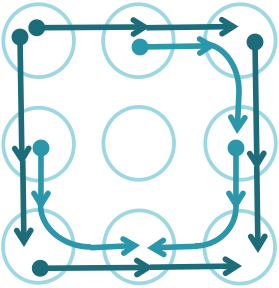
\includegraphics[width=0.31\textwidth]{pics/analysis/3gram1.png}
    }
    \subfigure{
      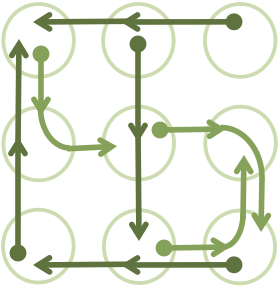
\includegraphics[width=0.31\textwidth]{pics/analysis/3gram2.png}
    }
    \subfigure{
      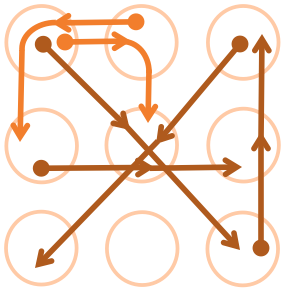
\includegraphics[width=0.31\textwidth]{pics/analysis/3gram3.png}
    }
    \caption{Most common 3-gram to less common 3-gram}
    \label{fig:3gram}
  \end{figure}

\subsection{Bias in the Selection of Start Node}

  %Table: Starting node dist
  \begin{table}[H]
    \centering
    \begin{tabular}{ c || c | c || c | c | c | c }
      \hline
      {\bf Start node} & All & 1,2,3 & 1 & 2 & 3 & T \\ \hline
      1 & 44\% & 42\% & 43\% & 41\% & 42\% & 51\% \\
      3 & 15\% & 15\% & 16\% & 14\% & 13\% & 14\% \\
      7 & 14\% & 14\% & 13\% & 15\% & 14\% & 13\% \\
      2 & 9\%  & 9\%  & 10\% & 9\%  & 8\%  & 7\%  \\
      4 & 6\%  & 7\%  & 6\%  & 7\%  & 7\%  & 6\%  \\
      5 & 4\%  & 4\%  & 4\%  & 4\%  & 4\%  & 3\%  \\
      9 & 4\%  & 4\%  & 3\%  & 3\%  & 5\%  & 3\%  \\
      8 & 2\%  & 3\%  & 2\%  & 3\%  & 3\%  & 2\%  \\
      6 & 2\%  & 2\%  & 2\%  & 2\%  & 3\%  & 2\%  \\ \hline
    \end{tabular}
    \caption{Starting node (1 = Shopping, 2 = Smartphone, 3 = Bank, T = Training)}
    \label{tab:startingNode}
  \end{table}

    %Figure: Staring node for all patterns
  \begin{figure}[H]
    \centering
    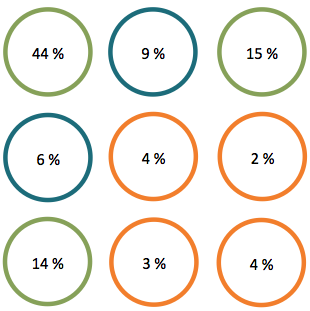
\includegraphics[scale=0.45]{pics/analysis/startingNode.png}
    \caption{Staring node for all patterns}
    \label{fig:startingNode}
  \end{figure}

  \clearpage

  \begin{figure}[H]
    \vspace{1.5cm}
    \centering
    \subfigure[Patterns created by right-handed respondents holding the smartphone in the right hand using the thumb]{
      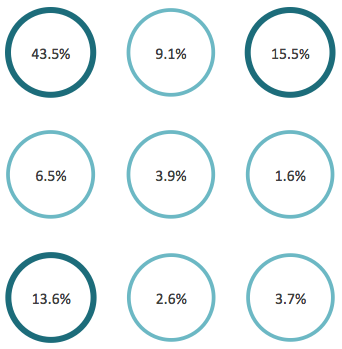
\includegraphics[width=0.45\textwidth]{pics/analysis/RRT.png}
    }
    \hspace{0.5cm}
    \subfigure[Patterns created by right-handed respondents holding the smartphone in the left hand using the forefinger]{
      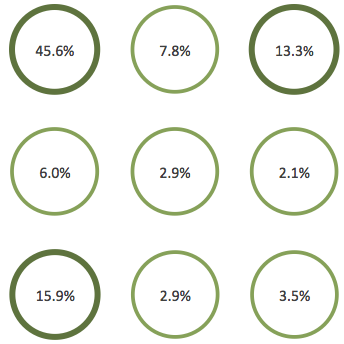
\includegraphics[width=0.45\textwidth]{pics/analysis/RLF.png}
    }
    \subfigure[Patterns created by left-handed respondents holding the smartphone in the left hand using the thumb]{
      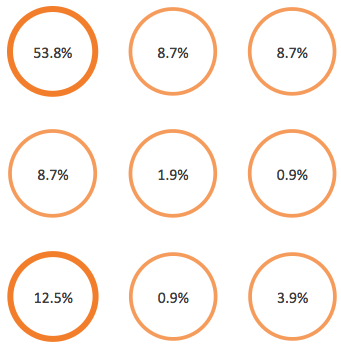
\includegraphics[width=0.45\textwidth]{pics/analysis/LLT.png}
    }
    \hspace{0.5cm}
    \subfigure[Patterns created by left-handed respondents holding the smartphone in the right hand using the forefinger]{
      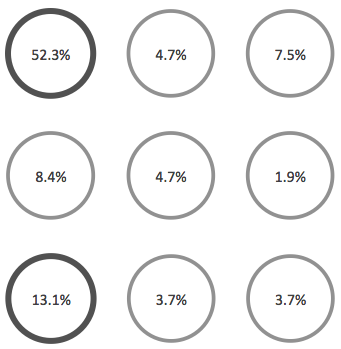
\includegraphics[width=0.45\textwidth]{pics/analysis/LRF.png}
    }
    \caption{Starting node based on handedness, hand used to hold smartphone, and finger used used when creating patterns}
  \end{figure}


\section{PIN codes vs. Android Unlock Patterns}
  
  \todo[inline, color=green!60]{PIN codes vs. Android Unlock Patterns. Få tak i PIN koder og sammenlige dem. Kan også beregne sannsynligheter. Sammeligne bruk. Sammeligne passwordspace. Frequency analysis of PIN codes. Snakke om at mange bruker PIN som er lett å taste inn eller PIN som er assosiert med feks en dato.}

  \begin{figure}[H]
    \centering
    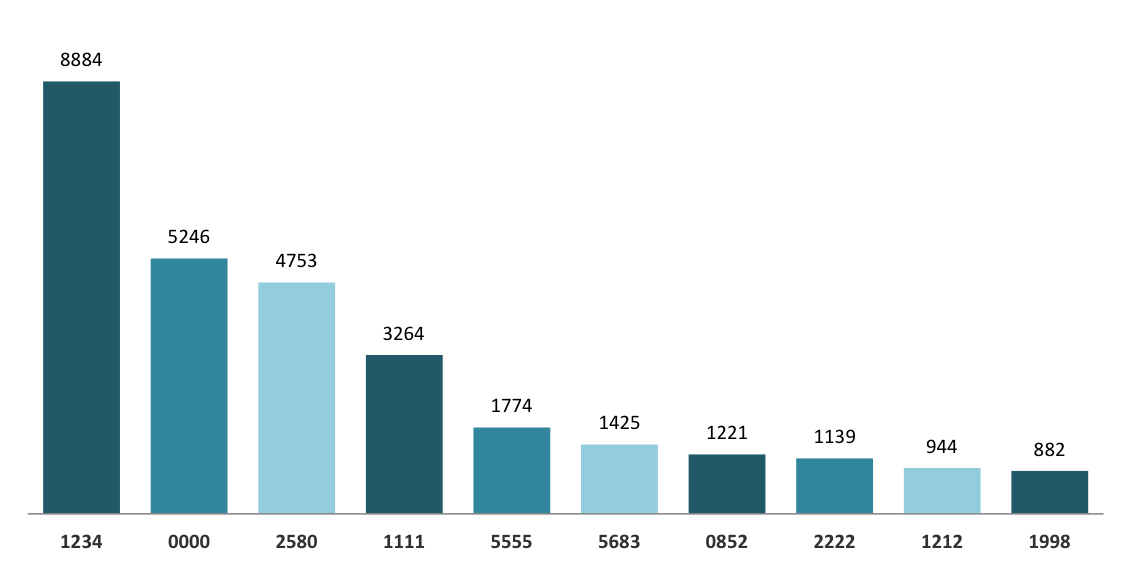
\includegraphics[width=\textwidth]{pics/analysis/top10pin.png}
    \caption{Top 10 PIN codes}
    \label{fig:top10pins}
  \end{figure}
    
  \begin{figure}[H]
    \centering
    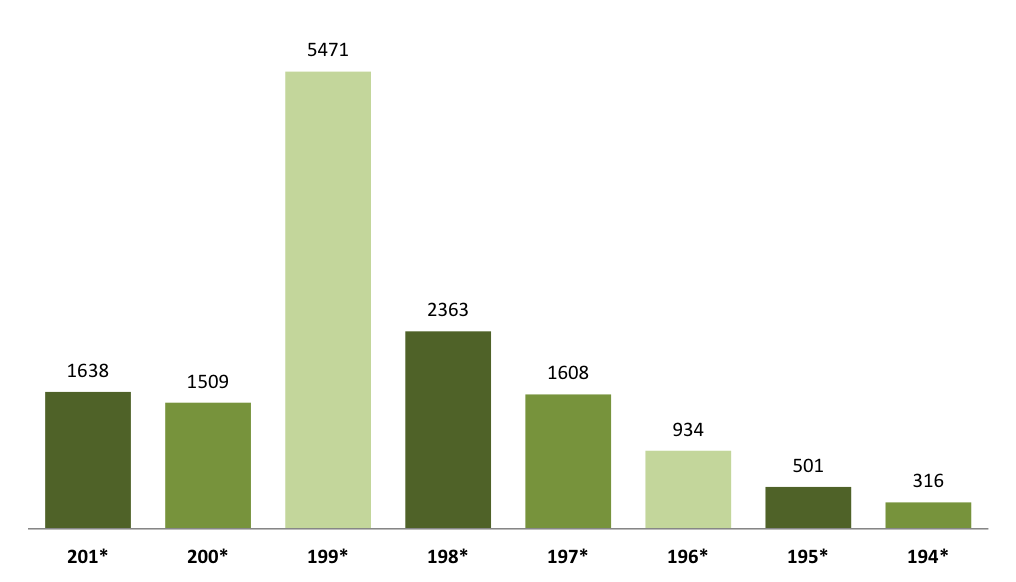
\includegraphics[width=\textwidth]{pics/analysis/pindecades.png}
    \caption{PIN codes by decade}
    \label{fig:pindecades}
  \end{figure}

  \begin{figure}[H]
    \centering
    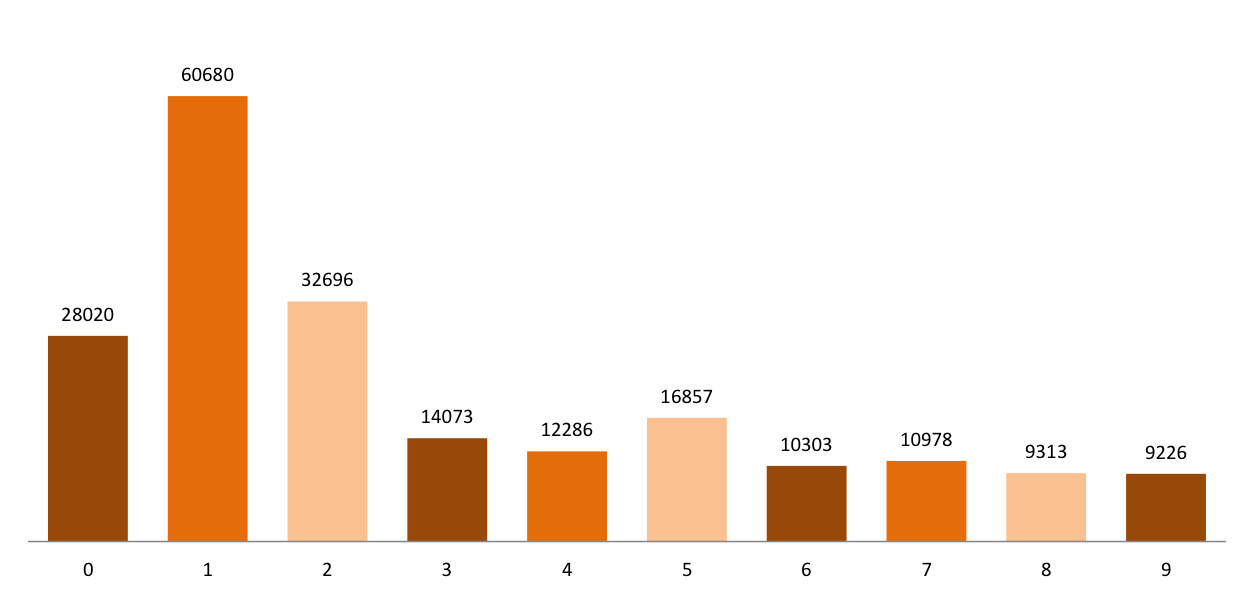
\includegraphics[width=\textwidth]{pics/analysis/pinstart.png}
    \caption{PIN code starting point}
    \label{fig:pinstart}
  \end{figure}

  \begin{figure}[H]
    \centering
    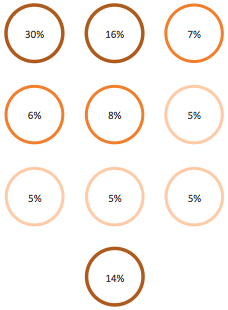
\includegraphics[width=0.40\textwidth]{pics/analysis/startpointpin.png}
    \caption{PIN code starting points}
    \label{fig:pinstart2}
  \end{figure}

  14.47 \% of the PIN codes was the top10 codes.






